\documentclass[a4paper,10pt]{article}
\usepackage{ESIEEcv}
\usepackage{graphicx}
\usepackage[french]{babel}
\usepackage[latin1]{inputenc}
\usepackage{color}
\definecolor{violet}{rgb}{0.35, 0.1, 0.35}
\definecolor{gris}{rgb}{0.4, 0.4, 0.4}

\oddsidemargin 0in

\advance\textwidth 125pt \advance\topmargin -0pt 
\textheight\paperheight \advance\textheight -2in \headheight 0pt
\headsep 0pt \footskip 0pt \voffset 0pt

\begin{document}
\vspace{-3.7cm}
\begin{center}
\textsc{\textbf{PhD}} \\
Robotics, Computer Science
%Sp�cialit� Informatique
\end{center}

\begin{minipage}{0.6\linewidth}
Sovannara \textsc{Hak}\\
10 all�e d'argoat \\
31770 Colomiers\\
FRANCE \\
Phone~: 06 81 13 47 04 \\
E-mail~: \texttt{hak.sovannara@gmail.com} \\
Homepage~: \texttt{http://homepages.laas.fr/shak/}
\end{minipage}
\begin{minipage}{0.4\linewidth}
\centering
\includegraphics[width=0.9in]{./me2.ps}\\
%\vspace{-0.37cm}
Date of Birth~: 8 December 1984 \\
Nationality~: French \\
\end{minipage} \\

%\vspace{-3.7cm}
%\begin{center}
%\textsc{\textbf{Sovannara HAK}} \\
%+33 6 81 13 47 04\\
%10 all�e d'argoat, 31770 Colomiers, FRANCE\\
%\texttt{hak.sovannara@gmail.com}, 
%\texttt{http://homepages.laas.fr/shak/}\\
%Date of Birth~: 8 December 1984 \\
%Nationality~: French \\
%\end{center}

\renewcommand{\FonteTitre}{\scshape}

\vspace{1.2cm}
\setlength{\largeurcolonne}{2.9cm}
\begin{rubrique}{\color{violet}Programming experiences}

\begin{sousrubrique}
\Date{November 2008} 
\Duree{3 years}
\Lieu{PhD Thesis, Toulouse - France} 
\Titre{LAAS (Laboratoire d'Analyse et d'Architecture des Syst�mes).}
\Descr{Title~: Task Recognition by reverse control}
\Apport{Development and implementation in C++ of a task recognition method based
on the control law of the robot for motion generation}
\Apport{Implementation of a solver to transfer motion capture data to joint angle 
trajectories for the HRP-2 robot}
\Apport{Implementation of an active waiting motion generator for the HRP-2}
\end{sousrubrique}

\begin{sousrubrique}
\Date{March 2008} 
\Duree{4 months}
\Lieu{Master Thesis, Orsay - France} 
\Titre{LIMSI (Laboratoire Informatique M�canique Sciences de l'Ing�nieur).}
\Descr{Title~: Paraphrase detection using syntactic context for question answering systems}
\Apport{Development and implementation in Perl and SQL of a method to detect paraphrases in a text corpus based on the 
syntactic relationship between the phrases of the sentences} 
%The main hypothesis is that
%sentences sharing similar contextual information tend also to share similar syntactic relationships.
%The syntactic relationships from the corpus are stored in a SQL database, and given a question in natural
%language, queries are generated in order to select candidates answers}
\end{sousrubrique}

\begin{sousrubrique}
\Date{April 2007} 
\Duree{6 months} 
\Lieu{Master Thesis, Tsukuba - Japan} 
\Titre{JRL (Joint Robotics Laboratory).}
\Descr{Title~: Generalized inverse kinematic and interaction for a humanoid robot}
\Apport{Implementation of generalized inverse kinematic algorithms in C++}
\Apport{Integration of a haptic device to allow an operator to drive the
inverse kinematic algorithms, through drag and drop manipulations}
\Apport{Experimentation with the model of a HRP-2 robot}
\end{sousrubrique}

\begin{sousrubrique}
\Date{June 2006} 
\Duree{3 months}
\Lieu{Technical Training, �vry - France} 
\Titre{Laboratoire IBISC (Informatique Biologie Int�gratives et Syst�mes Complexes).} 
\Descr{Title~: Inverse kinematic for a 6 DOF industrial robot and tele-operation in augmented reality and stereo-vision}
\Apport{Implementation in C++ of an analytical inverse kinematic for a 6 DOF Fanuc robot}
\Apport{Integration of an infrared optical tracking systems to control the virtual robot with a flying joystick}
\Apport{Development of an augmented reality application in stereo-vision to tele-operate the real robot in
a shape sorter game}
\end{sousrubrique}

\end{rubrique} 
\pagebreak
\begin{center}
\textsc{\textbf{Sovannara HAK}} \\
\end{center}

\begin{rubrique}{\color{violet}Education}
        \begin{sousrubrique}
                \Date{2008 - 2011} 
		\Titre{PhD in Robotics at INSA Toulouse (Institut National des Sciences Appliqu�es de Toulouse)}
                \Descr{Humanoid robots, movement analysis, task function formalism.}
                \Lieu{Toulouse - France}
        \end{sousrubrique}

        \begin{sousrubrique}
                \Date{2007 - 2008} 
		\Titre{Master of Science in Computer Science at Universit� Paris-Sud 11}
                \Descr{Natural language processing, natural speech recognition.}
                \Lieu{Orsay - France}
        \end{sousrubrique}

        \begin{sousrubrique}
                \Date{2004 - 2007}
                \Titre{Engineer degree at ENSIIE (Ecole Nationale Sup�rieure d'Informatique pour
                l'Industrie et l'Entreprise) recruiting through the Centrale-Sup�lec entrance examination}
                \Descr{Computer Science, robotics, virtual reality.}
                \Lieu{�vry - France}
                %$3^{e}$ ann�e, Options IA, Applications R�actives, R�seaux S�curit� et QoS.
                %\newline $2^{e}$ ann�e, Option Robotique et R�alit� virtuelle.}
        \end{sousrubrique}
\end{rubrique}
%\renewcommand{\FonteTitre}{\scshape}

%\pagebreak
%\begin{center}
%\textsc{Sovannara HAK} \\
%\end{center}
\renewcommand{\FonteTitre}{\scshape}
\begin{rubrique}{\color{violet}Technical Skills}
	\begin{sousrubrique}
		\Competence{OS} \Descr{Linux.}
	\end{sousrubrique}

	\begin{sousrubrique}
		\Competence{Programming} \Descr{C/C++, Matlab, Maple, shell script, Perl, Python, SQL.}
	\end{sousrubrique}
	
	\begin{sousrubrique}
		\Competence{Libraries} \Descr{Boost, STL.}
	\end{sousrubrique}
	
	\begin{sousrubrique}
		\Competence{Tools} \Descr{Git, Cmake.}
	\end{sousrubrique}
	
	\begin{sousrubrique}
		\Competence{Software} \Descr{Evart/Cortex, OpenHRP.}
	\end{sousrubrique}

	\begin{sousrubrique}
		\Competence{Other} \Descr{HRP-2 robot, Motion Analysis motion-capture system.}
	\end{sousrubrique}
\end{rubrique}

\begin{rubrique}{\color{violet}Languages}

	\begin{sousrubrique}
		\Competence{French} 
		\Descr{Native.}
	\end{sousrubrique}
	\begin{sousrubrique}
	  \Competence{English}
	  \Descr{Fluent. TOEIC 880/990 in 2006.}
	\end{sousrubrique}
	\begin{sousrubrique}
	  \Competence{Japanese}
	  \Descr{Beginner.}
	\end{sousrubrique}
\end{rubrique}

\begin{rubrique}{\color{violet}Interests}
  \begin{sousrubrique}
    \Competence{Music}
    \Descr{Self taught guitar player, DAW.}
  \end{sousrubrique}
\end{rubrique}

\pagebreak
\begin{center}
\textsc{\textbf{Sovannara HAK}} \\
\end{center}
\setlength{\largeurcolonne}{2.4cm}
\begin{rubrique}{\color{violet}Publications}
  \begin{sousrubrique}
    \Competence{Journal \newline Paper}
    \Descr{{\color{gris}\textbf{S. Hak}, N. Mansard, O. Stasse and J.P. Laumond ``Reverse Control for a Humanoid Robot Task Recognition", submitted in \emph{IEEE Transaction on Systems, Man, and Cybernetics Part B (TSMCB)}}}
  \end{sousrubrique}
  \begin{sousrubrique}
    \Competence{International Conference}
    \Descr{O. Ramos, L. Saab, \textbf{S. Hak} and N. Mansard, ``Dynamic Motion Capture and Edition
    using a Stack of Tasks", \emph{International Conference on Humanoid Robots (Humanoids), (Bled, Slovenia)}, October 2011}
  \end{sousrubrique}
  \begin{sousrubrique}
    \Descr{\textbf{S. Hak}, N. Mansard and O. Stasse, ``Humanoid robot task recognition from movement
    analysis", in \emph{International Conference on Humanoid Robots (Humanoids), (Nashville, USA)}, December 2010}
  \end{sousrubrique}
  \begin{sousrubrique}
    \Competence{National Conference}
    \Descr{\textbf{S. Hak}, N. Mansard and O. Stasse, ``Identification de T\^aches pour le Contr\^ole d'un Robot Humano�de", in \emph{Journ�es Nationales de la Robotique Humano�de, (Poitiers, France)}, June 2010}
  \end{sousrubrique}
\end{rubrique}

\renewcommand{\FonteTitre}{\scshape}
\begin{rubrique}{\color{violet}References}
  \begin{sousrubrique}
    \Competence{Jean-Paul Laumond}
    \Descr{Research director,\newline
    LAAS-CNRS Toulouse, France,\newline 
    E-mail~: \texttt{jpl@laas.fr}}
  \end{sousrubrique}

  \begin{sousrubrique}
    \Competence{Nicolas\newline Mansard}
    \Descr{Researcher,\newline
    LAAS-CNRS Toulouse, France,\newline 
    E-mail~: \texttt{nmansard@laas.fr}}
  \end{sousrubrique}

  \begin{sousrubrique}
    \Competence{Olivier Stasse}
    \Descr{Researcher,\newline 
    CNRS-AIST JRL, ISRI, Tsukuba, Japan,\newline
    E-mail~: \texttt{olivier.stasse@aist.go.jp}}
  \end{sousrubrique}

  \begin{sousrubrique}
    \Competence{Abderrahmane Kheddar}
    \Descr{Research director,\newline
    LIRMM-CNRS Montpellier, France,\newline
    E-mail~:\texttt{abderrahmane.kheddar@aist.go.jp}}
  \end{sousrubrique}
\end{rubrique}

\end{document}
